\documentclass[a4paper,titlepage,12pt]{article}
\usepackage[utf8]{inputenc} %Make sure all UTF8 characters work in the document
\usepackage{graphicx}
\usepackage{titling}
\usepackage{tabularx}
\usepackage{longtable}
\usepackage[yyyymmdd]{datetime}
\usepackage[figurename=Figur]{caption}
\usepackage{booktabs}
\usepackage[parfill]{parskip}
\usepackage[toc,page]{appendix}

%Set page size
\usepackage{geometry}
\geometry{margin=3cm}

\renewcommand{\dateseparator}{-}
\renewcommand{\contentsname}{Innehållsförteckning}
\renewcommand{\tablename}{Tabell}


\usepackage{listings}
\usepackage{color}

\usepackage[colorinlistoftodos,prependcaption,textsize=tiny]{todonotes}

\definecolor{dkgreen}{rgb}{0,0.6,0}
\definecolor{gray}{rgb}{0.5,0.5,0.5}
\definecolor{mauve}{rgb}{0.58,0,0.82}

\lstset{frame=tb,
  language=Python,
  aboveskip=3mm,
  belowskip=3mm,
  showstringspaces=false,
  columns=flexible,
  basicstyle={\small\ttfamily},
  numbers=none,
  numberstyle=\tiny\color{gray},
  keywordstyle=\color{blue},
  commentstyle=\color{dkgreen},
  stringstyle=\color{mauve},
  breaklines=true,
  breakatwhitespace=true,
  tabsize=3
}

%%%%%%%%%%%%%%%%%%%%%%%%%%%%%%%
% Header and footer
%%%%%%%%%%%%%%%%%%%%%%%%%%%%%%%
\usepackage{fancyhdr}
\pagestyle{fancy}

\lhead{
\includegraphics[width=0.15\linewidth]{../images/logo_full.png}}
\chead{Teknisk dokumentation för sexbent robot}
\rhead{\today}
\setlength\headheight{26pt} 

\lfoot{TSEA29 -- KMM \\ Teknisk Dokumentation}
\rfoot{Grupp 9 \\ LiTHe Hex}

\newcommand{\itc}{I\textsuperscript{2}C}

\pretitle{%
	\begin{center}
		\LARGE
		
\includegraphics[width=6cm]{../images/logo_full.png}\\[\bigskipamount]
}

\posttitle{\end{center}}

\begin{document}
\listoftodos
	\title{\LARGE
		\textbf{Teknisk dokumentation för sexbent robot} \\
		\vspace*{0.5\baselineskip}
		\large
		Redaktör Frans Skarman \\
		Grupp 9 \\
		\small
		\vspace*{0.5\baselineskip}
		Version 1.0}

	\date{\today}

	\maketitle
	
	\newpage
	
	\begin{center}

		%%%%%%%%%%%%%%%%%%%%%%%%%%%%%%%%%%%%%%%%%%%%%%%%%%%%%%%%%%%%%%%%%%%%%%%%%%%%%%%%%
		%						Medlemmar
		%%%%%%%%%%%%%%%%%%%%%%%%%%%%%%%%%%%%%%%%%%%%%%%%%%%%%%%%%%%%%%%%%%%%%%%%%%%%%%%%%

		\section*{Projektidentitet}
		Grupp 9, Ht 2016, LiTHe Hex

		Linköpings Tekniska Högskola, ISY

		\renewcommand*{\arraystretch}{1.4}
		\begin{longtable}[c]{ l l l }
			\textbf{Namn} & \textbf{Ansvar} & \textbf{E-post} \\ \midrule
			Emil Segerbäck & & emise935@student.liu.se \\ \midrule
			Frans Skarman & Dokumentansvarig & frask812@student.liu.se \\ \midrule
			Hannes Tuhkala & & hantu447@student.liu.se \\ \midrule
			Malcolm Vigren & Projektledare & malvi108@student.liu.se \\ \midrule
			Noak Ringman &  & noari093@student.liu.se \\ \midrule
			Olav Övrebö &  & olaov121@student.liu.se \\ \midrule
			Robin Sliwa &  & robsl733@student.liu.se \\
		\end{longtable}

		\centering
		\textbf{Kursansvarig}: Tomas Svensson Rum 3B:528 013--28 13 68 tomas.svensson@liu.se

		\newpage
		\tableofcontents
		\newpage


		%%%%%%%%%%%%%%%%%%%%%%%%%%%%%%%%%%%%%%%%%%%%%%%%%%%%%%%%%%%%%%%%%%%%%%%%%%%%%%%%%
		%						Historik
		%%%%%%%%%%%%%%%%%%%%%%%%%%%%%%%%%%%%%%%%%%%%%%%%%%%%%%%%%%%%%%%%%%%%%%%%%%%%%%%%%

		\section*{Dokumenthistorik}
		\renewcommand*{\arraystretch}{1.4}
        \begin{longtable}[c]{ l l >{\raggedright}p{5cm} >{\raggedright}p{3cm} l }
			\textbf{Version} & \textbf{Datum} & \textbf{Utförda förändringar} 
			& \textbf{Utförda av} & \textbf{Granskad} \\ \midrule
			
			0.1 & 2016--10--20 & Första utkastet & Projektgruppen &
            Projektgruppen \\
            
		\end{longtable}
	\end{center}

	%%%%%%%%%%%%%%%%%%%%%%%%%%%%%%%%%%%%%%%%%%%%%%%%%%%%%%%%%%%%%%%%%%%%%%%%%%%%%%%%%
	%						Inledning
	%%%%%%%%%%%%%%%%%%%%%%%%%%%%%%%%%%%%%%%%%%%%%%%%%%%%%%%%%%%%%%%%%%%%%%%%%%%%%%%%%

	\newpage

	\raggedright

	\section{Inledning}
	Detta dokument går i detalj in på konstruktionen och mjukvaran för en 
	sexbent robot, med autonom och manuell styrning. Först presenteras en 
	översiktlig beskrivning av robotens styrande processorer ("enheter", vilka kopplas till ett färdigt 
	PhantomX AX Metal Hexapod Mark III chassi från TrossenRobotics). Dessa enheter (central-, 
	motorik- och sensorenhet), kommunikation mellan dessa, samt användargränssnitt specificeras 
	sedan i större noggrannhet under egna avdelningar.

	%%%%%%%%%%%%%%%%%%%%%%%%%%%%%%%%%%%%%%%%%%%%%%%%%%%%%%%%%%%%%%%%%%%%%%%%%%%%%%%%%
	%						Översikt
	%%%%%%%%%%%%%%%%%%%%%%%%%%%%%%%%%%%%%%%%%%%%%%%%%%%%%%%%%%%%%%%%%%%%%%%%%%%%%%%%%

	\section{Systemöversikt}
	Systemet innehåller tre enheter. En centralenhet implementerad på en Raspberry Pi 3 
	agerar som master för de andra två (slav-)enheterna. Denna står för all kommunikation 
	med omgivningen genom en webbserver som datorer kan koppla upp sig mot för att styra roboten 
	eller få tillgång till debugdata. I autonomt läge är det även denna enhet som utifrån 
	insamlad data fattar alla styrande beslut utifrån vilka de andra enheterna 
	verkar. Vid manuell styrning vidarebefordras endast data från styrdatorn.

	De två andra enheterna (slavarna till centralenheten) utgörs av AVR-processorer och styr 
	mer generella uppgifter. Den ena, motorikenheten, översätter generella indikationer om 
	förflyttning från centralenheten till faktiska kommandon för robotens servon och skickar 
	vidare dessa. Den kan även förse centralenheten med bland annat debugdata om så efterfrågas.
	
	% Tror inte vi använde brusreducering va? Ta bort den delen
	% isf.
	Den andra AVR-processorn utgör en sensorenhet, vilken styr och läser robotens sensorsvit. 
	Den svarar även för att översätta råa sensordata till mer konkreta former (som vinklar och 
	avstånd), samt att brusreducera dessa efter behov. Figur \ref{fig:overview} ger en översiktsbild av
	systemet.
	
	% Ska det stå servon eftersom det står sensorer?
	\begin{figure}[h!]
		\centering
		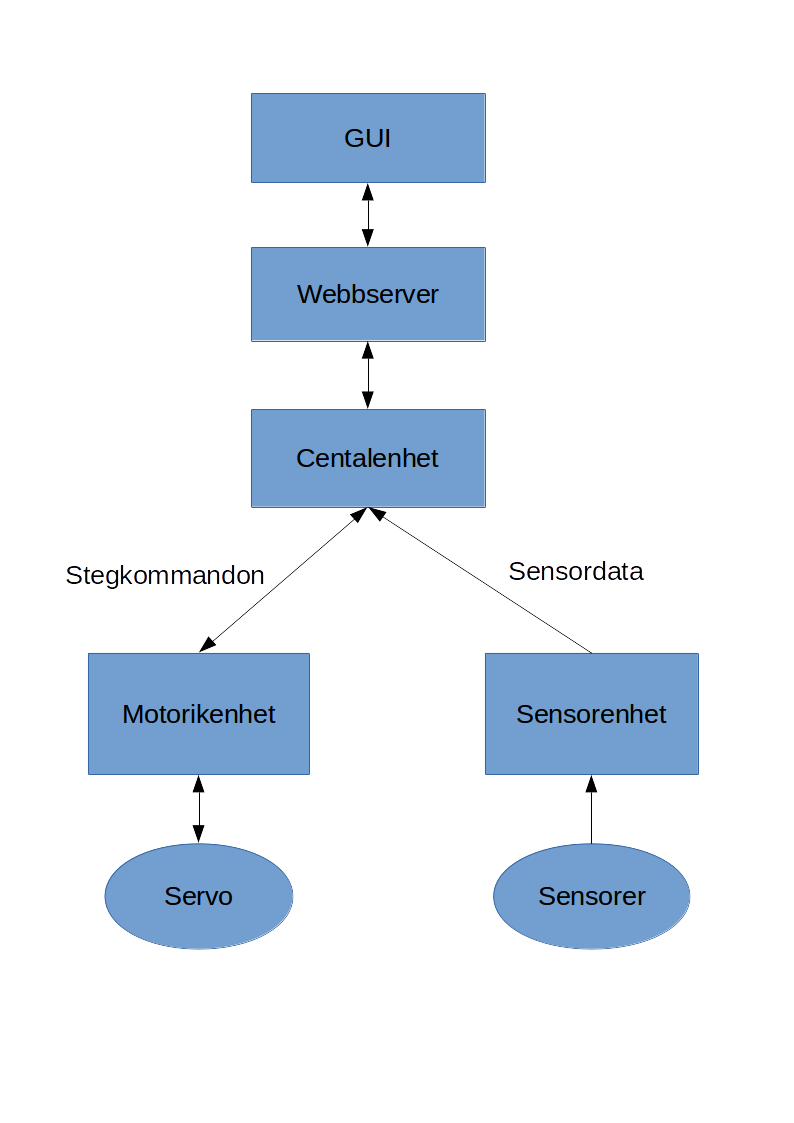
\includegraphics[width=0.5\linewidth]{../images/overview.png}
		\caption{Översikt av systemet\label{fig:overview}}
	\end{figure}

	\newpage

	\section{Kommunikation mellan enheterna}
	Kommunikation mellan centralenheten och de två AVR-processorerna sker
	med SPI. Sensor- och motorikenhetens SPI-portar är kopplade till varsin
	SPI-port på centralenheten. Detta illustreras i figur \ref{fig:central_circuit}.
	All kommunikation inleds med att centralenheten skickar ett kommando 
    eller en databegäran till slavenheterna.
	Slavenheterna utför sedan kommandot eller svarar med den begärda data.

	\begin{figure}[htpb]
		\centering
		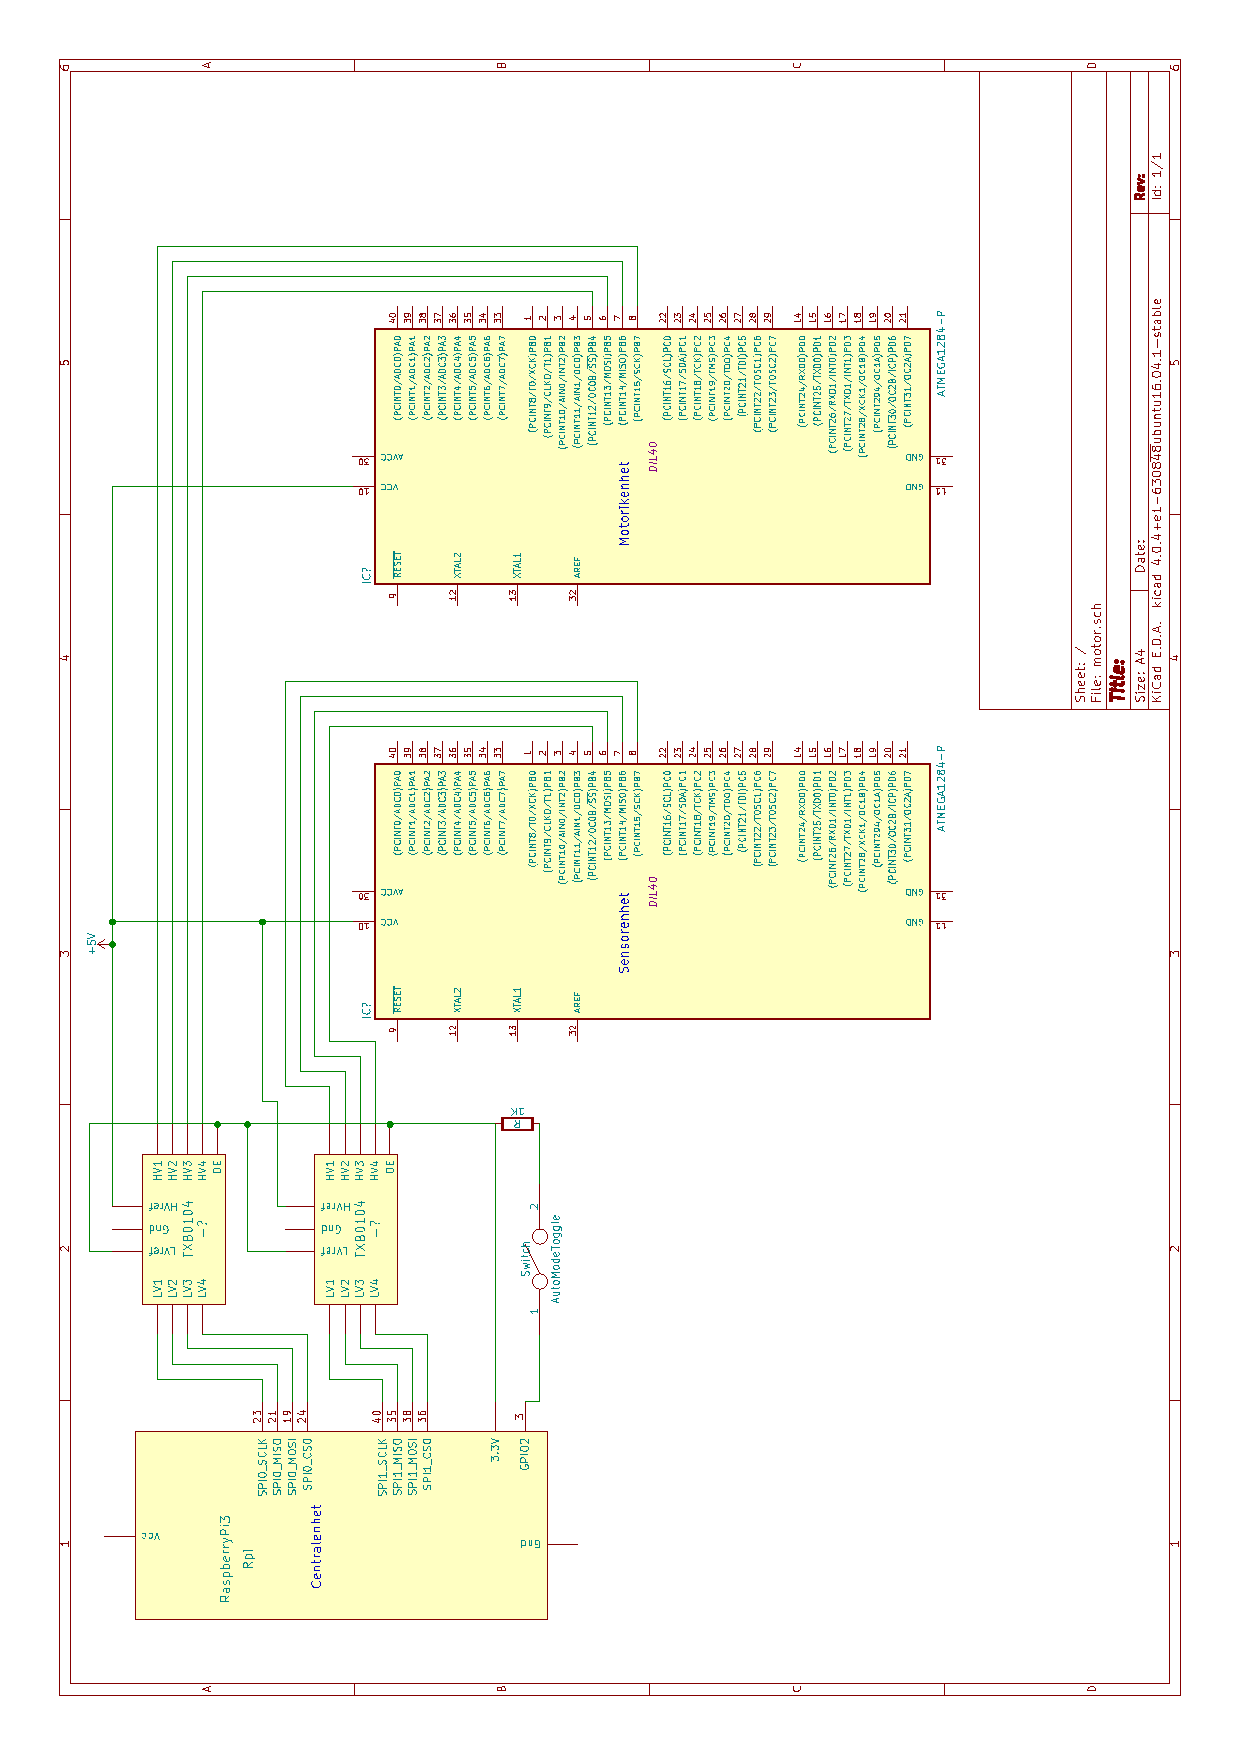
\includegraphics[width=1.0\linewidth]{charts/central/centralenhet.pdf}
		\caption{Kopplingsschema för centralenheten}
		\label{fig:central_circuit}
	\end{figure}




	\subsection{Kommunikationsprotokoll}
	\label{ssub:Kommunikationsprotokoll}
	Kommunikationen mellan centralenheten, motorikenheten och sensorenheten sker 
	med protokollet som beskrivs i figur \ref{fig:kommunikation1}.

	\newpage
	\begin{figure}[h!]
		\centering
		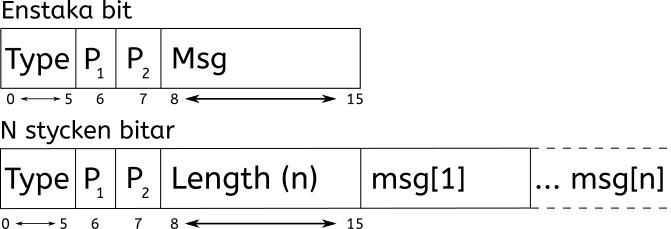
\includegraphics[width=0.5\linewidth]{images/communication_protocol1.png}
		\caption{Översiktlig vy av kommunikationsprotokolllet}
		\label{fig:kommunikation1}
	\end{figure}

	De första 6 bitarna av varje meddelande säger vilken typ av meddelande det är som
	skickas, dessa beskrivs i tabell 
	\ref{table:messages}. Den första biten i typparametern är 0 om meddelandets
	innehåll är en enstaka byte och 1 om meddelandet har dynamisk längd. Om längden
	är dynamisk är första byten i meddelandet längden av resten av meddelandet.

	De två sista bitarna i första byten är paritetsbitar. Bit 7 är en  paritetsbit
	för meddelandets innehåll medan bit 8 är paritetsbit för de 7 tidigare bitarna.

	Om någon av paritetsbitarna är fel så kommer enheten som tog emot meddelandet att svara
	med ett speciellt meddelande för att indikera sändningsfel. Annars kommer den 
	att svara med ett "acknowledgemeddelande".

    \newpage
	\begin{longtable}[c]{ l l l }
		\textbf{Syfte} & \textbf{ID} & \textbf{Data} \\ \midrule
		\textbf{Generella} \\ \midrule
		Send fail & 1F & -- \\ \midrule
		Acknowledge & 0F & -- \\ \midrule
		Datarequest & 02 & data \\ \midrule
		\\
		\textbf{Centralenhet $ \to $ motorikenhet}\\ \midrule
		Sätt hindergång & 03 & på/av \\ \midrule
		Sätt servohastighet & 20 & 8 LSD, 8 MSD \\ \midrule
		Gåkommando &  21 & len, x- och y-hastighet, svänghastighet,
        autonom-läge \\ \midrule
		Return to neutral & 05 & -- \\ \midrule
		\\
		\textbf{Centralenhet $ \gets $ motorikenhet}\\ \midrule
		Servostatus & 22 & len, ... data ... \\ \midrule
		Debugsträng & 23 & len, "debugsträng i utf-8" \\ \midrule
		Upptagen med rotation? & 03 & ja: 0x01, nej: 0x00 \\ \midrule
		\\
		\textbf{Centralenhet $\to$ sensorenhet} \\ \midrule
		Återställ orientering & 03 & -- \\ \midrule
		\\
		\textbf{Centralenhet $ \gets $ sensorenhet}\\ \midrule
		Behandlad sensordata & 24 & len,ir-ner, ir-fv, ir-bv, ir-fh, ir-bh,
        lidar-lsd, lidar-msb \\ \midrule
		Korridordata		 & 25 & len, avst. fram, vänster, höger, ned, vinkel \\

		\caption{Meddelandespecifikation \label{table:messages}}
	\end{longtable}
    
    \subsection{Centralenheten}

    Centralenheten använder SpiDev-modulen för python för kommunikation med
    motorik- och sensorenheten över SPI. Den skapar en instans av SpiDev för
    varje enhet, då centralenheten använder två separata SPI-bussar för varje
    enhet. Alla funktioner i som rör kommunikationen till AVR-processorerna tar
    alltså in instansen för den enhet som ska kommuniceras till.

    Pseudokoden för läsning av spi-meddelanden beskrivs som följande:

	\begin{lstlisting}
	def read_bytes(spidev):

		type_byte = spidev.read_single_byte()

        if is_multibyte_msg(type_byte):
            length_byte = spidev.read_single_byte()
            return spidev.read_several_bytes(length)
        else:
            return spidev.read_single_byte()

	\end{lstlisting}

	Algoritmen för att skicka data till AVR-processorerna ser lite annorlunda
    ut beroende på vad som ska skickas. Det som är gemensamt med alla
    transaktioner till enheterna är dock att först skickas en \textit{garbage}-byte
    (definierad 0x00) som ska ignoreras,
    då AVR-processorerna inte alltid lyssnar på den första 
    byten. Ifall AVR-processorerna märker att den första byten är en
    \textit{garbage}, så struntar de alltså i den, annars behandlar den
    meddelandet som vanligt. Det betyder att inga data-ID:n kan ha samma
    värde som \textit{garbage}-byten.

    Efter att \textit{garbage}-byten är skickad, skickar enheten hela
    meddelandet enligt protokollet, alltså genom att beräkna och lägga till
    paritetsbitar i byten för data-ID, skicka längden ifall det är flera bytes
    i meddelandet, och slutligen skicka de bytes som ska skickas.

	Algoritmen för mottagning och behandling av meddelanden på motorik- och
    sensorenheten körs i en avbrottsruting som beskrivs av följande pseudokod:

	\begin{lstlisting}
        def on_spi_interrupt():
			
            received_frame = receive_frame()
            success = check_parity(received_frame)

            if success:
                send_acknowledge_message()
            else:
                send_fail_message()
                return

            if received_frame.type == DATA_REQUEST:
                # message requires reply
                reply_frame = build_reply_frame()
                send_frame(reply_frame)
            else:
                # message contains command to be processed
                handle_frame(received_frame)

	\end{lstlisting}
    \textit{Frame} syftar på en datastruktur som innehåller all relevant
    information om meddelandet. som typ, längd och data

	\section{Komponentbudget}

    Tabell \ref{table:components} visar komponenter som ingår i
    roboten, utöver chassiet, lödplattor och andra diverse
    mindre komponenter.

	\begin{longtable}[c]{l l}
		\textbf{Komponent} & \textbf{Antal} \\ \midrule
		Raspberry Pi 3 & 1 \\
		ATmega1284 & 2 \\
		GP2D120 & 1 \\
		GP2Y0A02YK & 4 \\
		MLX90609 & 1 \\
		LIDAR Lite V3 & 1 \\
	    74LS240 & 8 \\
        Extern 16 MHz-klocka EXO-3 & 1 \\
        TXB0104 & 2 \\
        \caption{De komponenter som beräknas att gå åt \label{table:components}}
	\end{longtable}
	
    \newpage
	\section{Centralenheten}
        Centralenheten har två ansvarsområden: navigation/beslutsfattning samt
        kommunikation med omvärlden. Detta görs i två lägen, manuellt och autonomt
        läge. För att byta mellan dessa två lägen kan man antingen använda sig av den
        fysiska knappen eller knappen i användargränssnittet.

	\subsection{Navigation och beslutsfattning}
	Centralenheten sköter all beslutsfattning om hur roboten ska röra sig
	genom labyrinten. Den tar emot data från sensorenheten och GUI:t och
	skickar kommandon till motorikenheten.
  
	\subsubsection{Autonomt läge}
	\label{sec:central-autonom} 
	I det autonoma läget frågar centralenheten om data från sensorenheten
    varje gång det ska fattas ett beslut. Detta gör att centralenheten själv
    bestämmer när den ska ha ny data för att den inte ska bli avbruten eller missa
    data för att den är mitt i utförandet av en annan funktion. Utifrån denna data
    fattar centralenheten beslut om hexapodens färdriktning.

    I beslutsfattning ingår bland annat korridorreglering, svänga in i korridorer samt detektera
    och undvika återvändsgränder. Beslutsfattningen innehåller en lista med de tre senaste besluten och det är endast när alla dessa beslut är samma som beslutet uträttas. 
    
    Korridorregleringen sker med hjälp av de fyra IR-sensorerna som sitter på
    sidorna av roboten. En vinkel räknas ut med data från dessa som säger
    hur roboten är vinklad i en korridor. Regleringen sker samtidigt som när
    roboten går framåt för att få jämnare gång i korridoren. Detta uppnås genom
    att en offset från mitten av korridoren beräknas och används när roboten ska
    vrida sig tillbaka till mitten. Ju närmare mitten den är desto mindre kommer
    den att vrida sig mot mitten.

    \todo{Lägg till pseudokod för korridorreglering}%
    \begin{lstlisting}
    def regulate(sensor_data, decision_packet):
    \end{lstlisting}

    Förutom de fyra IR-sensorerna på sidorna används även LIDAR när beslut ska fattas. LIDAR-sensorn som är riktad framåt används
    för att undvika ingång i återvändsgränder framåt. När ett beslut om korridor
    eller återvändsgränd fattas används sidosensorerna för att detektera och
    bekräfta det som detekterats. Inget beslut fattas innan båda sidosensorerna
    har detekterat samma sak så att risken för felbeslut minskar.

    När ett beslut om vändning har tagits väntar koden tills att en hel vändning
    har skett. Detta görs genom att vänta tills roboten står rakt framåt m.h.a.
    den uträknade vinkeln men även genom att vänta tills motorikenheten svarar
    att en hel vändning har gjorts klart. När en hel vändning har skett går
    roboten framåt tills den har kommit in i den nya korridoren innan den börjar
    fatta beslut med sensordata den får in. Detta för att ignorera korridoren
    som roboten kom från. Se pseudokoden nedan. 
    
    \begin{lstlisting}
    def get_decision(sensor_data, decision_packet):
        corridors_and_dead_angles = get_corridors_and_dead_angles(sensor_data)

        for value in corridors_and_dead_ends:
            if 3 corridors detected:
                decision = TURN_LEFT
            
            elif 2 corridors detected:
                if distance forward is greater than DEAD_END_DISTANCE:
                    decision = GO_FORWARD
                else:
                    if left corridor detected:
                        decision = TURN_LEFT
                    else:
                        decision = TURN_RIGHT
            
            elif 1 corridor detected:
                if distance forward smaller than one tile 
                   and greater than LIDAR_STOP_DISTANCE:
                   decision = GO_FORWARD
                elif left corridor detected:
                    decision = TURN_LEFT
                elif right corridor detected:
                    decision = TURN_RIGHT
                else:
                    decision = GO_FORWARD

            elif 0 corridors detected:
                if distance forward is greater than LIDAR_STOP_DISTANCE:
                    decision = GO_FORWARD
                else:
                    decision = TURN_LEFT
    
    if previous decision is TURN_LEFT or TURN_RIGHT:
        # A complete turn has been made
        if absolute value of the average angle is less than 10 degrees and
        turn has completed:
            decision = GO_FORWARD
            previous_decision = COMPLETE_TURN

    elif previous decision is COMPLETE_TURN:
        decision = GO_FORWARD
        previous_decision = COMPLETE_TURN
        
        # if the robot has entered the new corridor
        if robot is inside a corridor:
            previous_decision = GO_FORWARD
        
    \end{lstlisting}
    
    \subsubsection{Manuell navigation}
    För den manuella navigationen används RabbitMQ som är en kommunikationsserver mellan webbservern
    och centralenheten. Det kommer in ett nytt meddelande med data för varje
    knapptryck/händelse som sker på GUI:t som centralenheten tolkar och överför
    till motorikenheten.

	\subsection{Kommunikation}
	Centralenheten kommunicerar med en dator över WiFi. Datorns webbläsare 
	ansluter till centralenhetens webbserver och då kan man
	via webbgränssnittet styra roboten samt läsa av robotens olika data. 
		
	\subsubsection{Kommunikation med webbserver}
	Centralenheten skickar och hämtar kontinuerligt meddelanden ifrån RabbitMQ servern och är i JSON-format. Centralenheten skickar den data som GUI:t
	behöver till RabbitMQ servern och webbservern läser sedan in den data som finns där.
	Den data som skickas mellan centralenheten till webbservern kan ses i
	tabell \ref{table:guimessagesfromcentral} och den data som skickas från webbservern till centralenheten kan ses i tabell \ref{table:guimessagestocentral} vid sektion \ref{gui:kommunikation}.

	% TODO: Den ger fel sektion ovan! Det ska vara 7.4 och inte 7.3.

	%%%%%%%%%%%%%%%%%%%%%%%%%%%%%%%%%%%%%%%%%%%%%%%%%%%%%%%%%%%%%%%%%%%%%%%%%%%%%%%%%
	%						Motorikenheten
	%%%%%%%%%%%%%%%%%%%%%%%%%%%%%%%%%%%%%%%%%%%%%%%%%%%%%%%%%%%%%%%%%%%%%%%%%%%%%%%%%
    \newpage
	\section{Motorikenheten}
	Motorikenheten översätter kommandon från centralenheten till servokommandon. Den tar emot 
	instruktioner från centralenheten som anger steglängd, fart, rotation och riktning för 
	förflyttnnig. Motorikenheten behandlar detta, räknar ut en lämplig gångstil och 
	signalerar nödvändiga vinklar till de sex benen. Vissa delmoment i förflyttningen 
	görs hårdkodade. Ett kretschema för motorikenheten finns i figur \ref{fig:motorik}.

	För att kunna kommunicera med servona i 1 MBAUD klockas motorikenheten med en 16 MHz 
	EXO3 klocka.

	\begin{figure}[htpb]
		\centering
		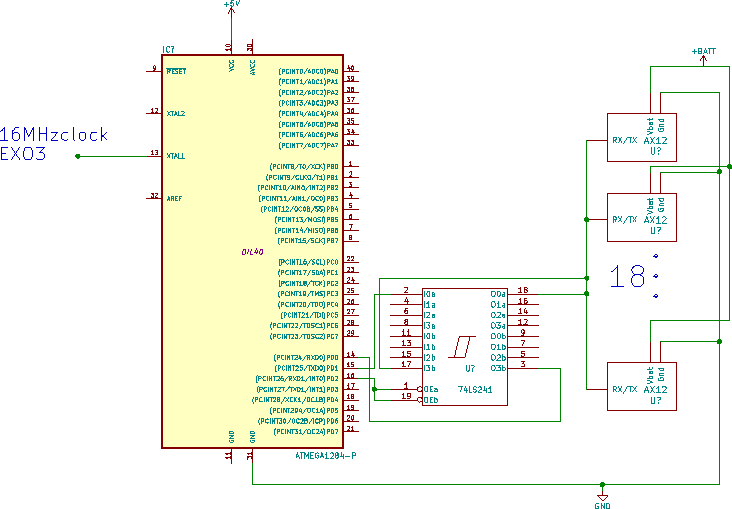
\includegraphics[width=1.0\linewidth]{charts/motor/motorik.pdf}
		\caption{Kretsschema för motorikenheten}
		\label{fig:motorik}
	\end{figure}
	
		\subsection{Kommandotolkning}
	Motorikenheten  tar in ett flyttalspar med koordinater för önskad målposition (önskat 
	center för roboten efter förflyttning), med x-koordinat fram och 
	y-koordinat åt vänster om roboten, och med origo i robotens mittpunkt. Om totalavståndet 
	origo till målposition är mindre än 1 enhet skalas rörelsen ned utifrån detta avstånd. 
	Det vill säga, om roboten ombeds gå 0,5 enheter framåt, tar den ett kliv med halva 
	steglängden av om den ombetts gå en meter, även om inget av kliven är i närheten av 
	de respektive distanserna; om en enhetsdistans (maximal steglängd) leder till ett 
	1,6 decimeters kliv, leder halva ehtetsdistansen till ett ca: 0.8 decimeters kliv givet samma 
	startposition och riktning. 
	
	Vidare ges den rotation som roboten 
	skall rotera, angiven positiv vänster med 0 frammåt, och en flagga för om 
	roboten är i autonomt läge eller manuellt styrt läge. Om roboten är i autonomt läge, tolkas 
	rotation utan koordinater som att en strikt rotation skall utföras (det vill säga, att 
	roboten inte skall ändra rörelse förrän den utfört rotationen i fullo). I alla andra fall 
	tar roboten in ett nytt kommando efter att ett enda steg utförts i indikerad riktning. 
	%kontrollera att nedanstående stämmer, servospeedmanupulation inte implementerat at time of writing.
	Även robotens servohastighet styras utifrån ett fartvärde. 

		\subsection{Planläggning och utförande}
	Första steget i motorikenheten för en anpassad gångstil är att utifrån efterfrågad
	förflyttning avgöra en önskad slutposition för respektive ben, som för roboten närmare 
	det läge indikerat av centralenheten. Sedan avgörs den nedskalning av rörelsen som för 
	varje set om tre ben (vänster-, höger-, vänster-ben och höger-, vänster-, höger-ben, taget 
	frammifrån bakåt) är nödvändig för att robotbenen skall kunna nå positionen utan att ben 
        skär varandra, och utan att gå utanför benens räckvidd eller in under roboten. Skalningen 
        görs först utan rotation, så att målförflyttningen är precist uppnåbar, varefter omberäkning 
        och skalning görs med rotation och ny, nedskalad målposition, så att rotationen inte skall 
        försvinna i nedskalning gjord i första hand för förflyttningens skull. Denna dubbla skalning 
        görs två gånger, en med vardera uppsättning ben höjd, och roboten använder sig av det 
        alternativ där markfästa bens förflyttning är störst för att omberäkna benrörelsen, då dessa 
        ger den faktiska förflyttningen av chassit. 

	Beräkning av nedskalning sker i tre avseenden. För det första skalas benförflyttningarna 
	ner så att de inte tar benen utanför benens räckvidd. För det andra skalas  rörelserna så 
	att de inte skär en uppsättning hårdkodade gränser mellan ben och mellan fot och robotchassi.
	Avslutningsvis görs en nedskalning utifrån angivet kommando, så att steglängd kan justeras av 
	användaren. Om ingen rörelse anges, kommmer roboten att förbli stillastående. %och om den rörelsen som anges anses allt för svårutförd, kommer roboten att först anta en mer neutral ställning varifrån rörelsen bör vara utförbar.

	Bestämningen av benposition sker endast i planet; höjdled tas i beräkning endast inför åberopning 
	av IK, för bestämning av servovinklar. Själva klivet sker genom en sekvens av 
	positionsinställningar med höjning och sänkning av ben, och stegvis övergång från gällande till 
	önskad position. Vidare anpassas servonas aktuationshastighet för att ge en unison rörelse 
	över alla ben (hanterat i kommandot för servohandling). För en översiktlig inblick i 
	gångstilen, se figur \ref{fig:walkflow0}. Figuren visar beteendet specifikt i manuellt läge;
	i autonomt läge tillkommer möjligheten att med ett funktionsanrop rotera en strikt vinkel.
	Detta görs genom att upprepade åberopningar av koden för ensamt steg, illustrerat i figuren, 
	vilken returnerar andelen av det begärda klivet som uppnåtts.
	
	%start exempel pseudokod, som referens. Ta bort.
	%def get_decision(sensor_data, decision_packet):
    %    corridors_and_dead_angles = get_corridors_and_dead_angles(sensor_data)

    %    for value in corridors_and_dead_ends:
    %        if 3 corridors detected:
    %            decision = TURN_LEFT
    %        
    %        elif 2 corridors detected:
    %            if distance forward is greater than DEAD_END_DISTANCE:
    %                decision = GO_FORWARD
    %            else:
    %                if left corridor detected:
    %                    decision = TURN_LEFT
    %                else:
    %                    decision = TURN_RIGHT
	%end exempel pseudokod, som referens. Ta bort.
    	Nedan finns pseudokod för den mainloop som körs på motorikenheten. Besluten fattas 
	utifrån en struct som ändras av SPI via interrupts.

	\begin{lstlisting}
	def motorik_mainloop():
        stand_robot

        while true:
            if should move or rotate:
                if autonomous and only rotation:
                    rotate_until_done
                else
                    take_one_step_in_requested_direction
	\end{lstlisting}
	
    Vidare beskrivs nedan förenklat funktionaliteten för
    \textit{work\_towards\_goal} i gangstil.c, i pseudokoden skriven 
    som \textit{take\_one\_step\_in\_requested\_direction} för tydlighet:

	\begin{lstlisting}
	
	def take_one_step_in_requested_direction(rotation, goal_position, current_leg_placement):
		scale_down_leg_movement_to_executable(no_rotation, leg_set_1_raised, goal_position)
		scale_down_leg_movement_to_executable(rotation, leg_set_1_raised, downscaled_goal_position)

		scale_down_leg_movement_to_executable(no_rotation, leg_set_2_raised, goal_position)
		scale_down_leg_movement_to_executable(rotation, leg_set_2_raised, downscaled_goal_position)

		if(leg_set_1_raised_movement > leg_set_2_raised_movement):
			execute_scaled_movement(leg_set_1_raised)
		else:
			execute_scaled_movement(leg_set_1_raised)
		return downscale_of_movement
	\end{lstlisting}

	% TODO: Fix "typos" in figure
	\begin{figure}[h]
		\centering
		\includegraphics[width=0.5\linewidth]{images/gangstil_flowchart.png}
		\caption{Flödesschema för normal gångstil hos roboten
        \label{fig:walkflow0}}
        %TODO: Chart slightly out of date, update
	\end{figure}

	\subsection{Inverterad kinematik}
	\label{sub:inverterad-kinematik}
	Då planläggningsdelen av motorikenheten beslutat om var ett ben skall flyttas beräknas 
	lämpliga vinklar för benets alla servon genom inverterad kinematik. Utifrån kända 
	längder på benen och positioner där man vill att fötterna ska placeras används 
	trigonometri för att avgöra slutgiltiga servovinklar.
	
	% TODO: Fix image by making it bigger and adding z, x, y..
	% or remake it
	Inverterad kinematik är ett 3D-problem men vi har delat upp det i två
    stycken 2D-problem istället. Y-axeln går rakt upp, x-axeln går rakt ut från
    roboten i benfästets riktning och z-axeln går i riktningen $x \times y$
    längs med roboten. Det första 2D-problemet beräknar vinkeln mellan roboten
    och den innersta leden $\gamma$, det andra 2D-problemet beräknar vinkeln
    $\alpha$ mellan den första och andra leden samt vinkeln $\beta$ mellan den
    andra och tredje leden. Se figur \ref{fig:ik}.
	
	% Add formulas for the different angles?
	
	\begin{figure}[h!]
		\centering
		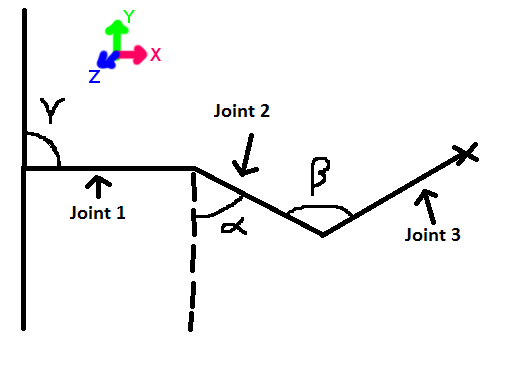
\includegraphics[width=0.5\linewidth]{images/ik.png}
		\caption{3D-problemet för IK med ett ben
		\label{fig:ik}}
	\end{figure}

	\subsection{Kommunikation med servon}
	Kommunikation med servona sker via en half-duplex UART-länk. AVR-processorns RX
	och TX pinnar är kopplade till var sin port på 74LS241 tri-state-grind. Portens riktning
	styrs med en vanlig IO pinne på processorn som sätts till HIGH när data ska skickas 
	och LOW när data tas emot. 

	\subsubsection{Skrivning av data}
	För att undvika onödiga svar från servona skrivs data till dem med hjälp av REG\_WRITE
	instruktionen som sparar data i en buffer på servot tills en ACTION instruktion skickas.
	Actioninstruktionen skickas med funktionen send\_servo\_action.
	
	\subsubsection{Läsning av data}
	För att läsa data från servona används funktionen read\_servo\_data som skickar en 
	databegäran till servona och läser resultatet. Begäran görs med hjälp av en
	READ\_DATA instruktion där addres och mängd bitar som ska läsa specificeras.
	
	Datan som returneras sparas i en struct som innehåller fält för metadata 
	(ID, errorflaggor, längd etc.) samt en array som innehåller den lästa datan.
	
	\subsubsection{Väntning på servorotation}
	För att inte behöva gissa hur lång tid ett steg kommer att ta så returnerar inte
	send\_servo\_action fören alla servon är nära sin målvinkel. Vad som räknas som "nära"
	beror på vilken del av steget som utför och skickas som parameter till 
	send\_servo\_action.

	För att se när rotationen är klar läses först varje servos nuvarande målvinkel in och
	sparas i en array. Varje servos nuvarande vinkel läses sedan in och jämförs med målet.
	Om skilnaden mellan nuvarande vinkel och målvinkel är under gränsen för "närhet" för
	varje servo så räknas rotationen som klar och funktionen returnerar.

	\subsubsection{Undantag för kommunikation}
	På grund av ett okänt fel i hård- eller mjukvaran blir UART signalen fel om data 
	begärs från de 3 första servona på roboten en bild på fenomenet kan ses i figur 
	\ref{fig:servo_tri_state_bug}. Eftersom att flera ben kommer att göra ungefär samma 
	rörelser samtidigt ignoreras därför de tre första servona vid beräkningar där data
	från servona behövs.

	\begin{figure}[htpb]
		\centering
		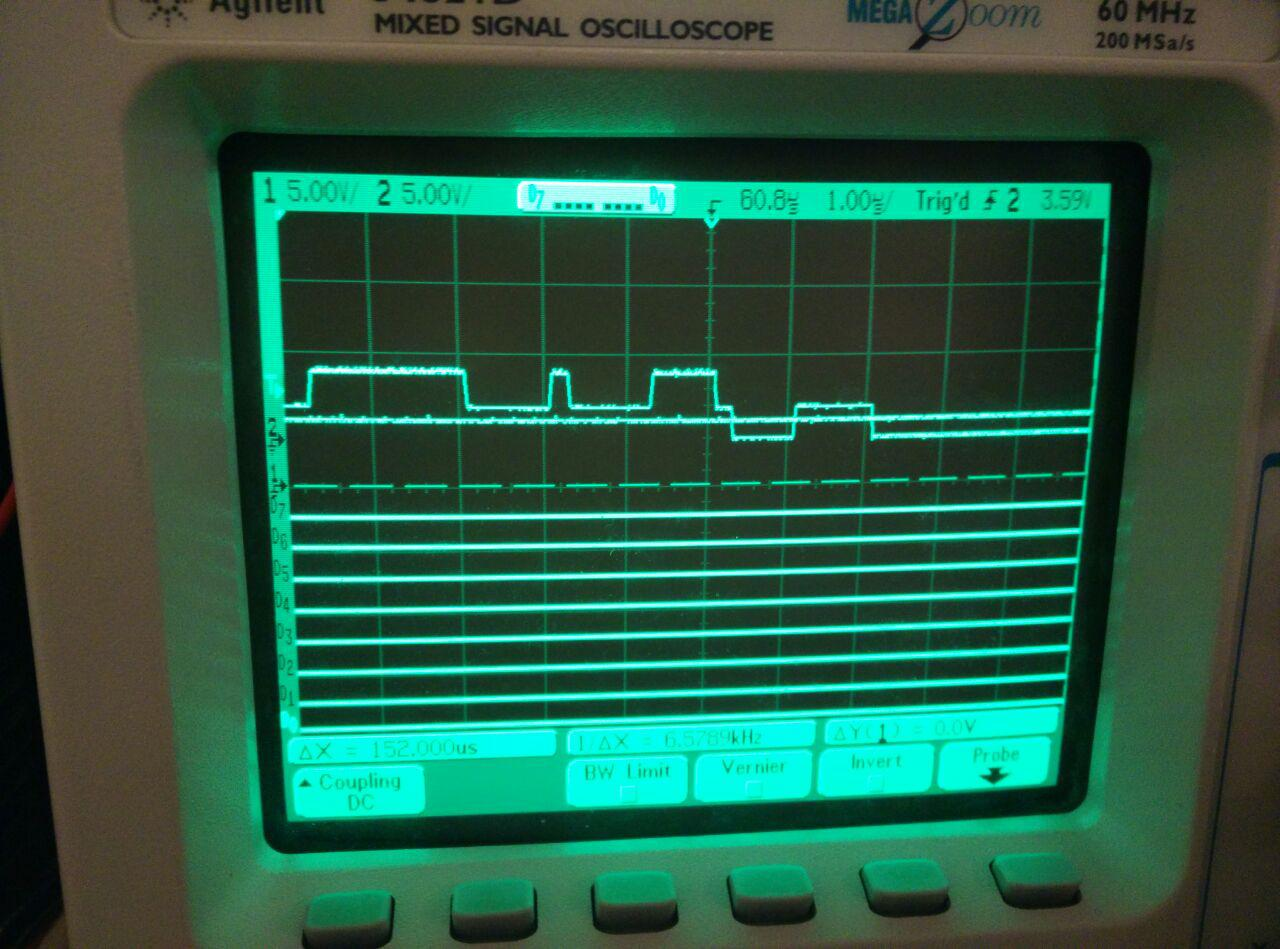
\includegraphics[width=0.8\linewidth]{images/uart_tri_state.jpg}
		\caption{UART signal när svar begärs från de tre första servona. 
			Signalen som skiftar mellan 3 lägen ska vara en digital signal}
		\label{fig:servo_tri_state_bug}
	\end{figure}


	%%%%%%%%%%%%%%%%%%%%%%%%%%%%%%%%%%%%%%%%%%%%%%%%%%%%%%%%%%%%%%%%%%%%%%%%%%%%%%%%%
	%						Sensorenheten
	%%%%%%%%%%%%%%%%%%%%%%%%%%%%%%%%%%%%%%%%%%%%%%%%%%%%%%%%%%%%%%%%%%%%%%%%%%%%%%%%%
	\section{Sensorenheten}
	Sensorenheten är den enhet som ger roboten sinnen för omvärlden, så att den
	kan navigera autonomt genom labyrinten. Sensorenheten sköter allting som
    rör läsning och brusreducering av sensorerna, och skickar dem till
    centralenheten på begäran.

	\subsection{Styrenhet i sensorenheten}
	Styrenheten för sensorenheten består av AVR-processorn ATmega1284, som läser av och 
	behandlar informationen från robotens sensorer. Styrenheten sköter även
	kommunikationen med centralenheten -- den tar emot förfrågningar om data och
	skickar behandlad data på begäran.

	Styrenheten behandlar den råa sensordata till den grad att
	centralenheten inte behöver göra allt för många egna beräkningar på
	sensorinformationen. Den sköter därför bland annat brusreducering av
	data. ATmega1284 har tillräckligt med 
	beräkningskraft för att ta hand om den data som sensorerna genererar. Den kritiska 
	delen är istället A/D-omvandling. Eftersom vi har många IR-sensorer tar det tid att 
	mäta och omvandla de analoga signalerna till digitala värden. Att starta en IR-sensor 
	tar 52 900 mikrosekunder och en A/D omvandling kan ta upp till 260 mikrosekunder. 

    \subsubsection{Huvudloop}
    Sensorenheten kör en huvudloop som hanterar en kö som varje ir-sensor är placerad 
    i. Den första ir-sensorn i kön är den första sensorn som kommer att ha ett nytt 
    värde. Tiden sedan förra mätningen av IR-sensorn beräknas och det är inte 
    möjligt att läsa en IR-sensor innan tiden passerat. Om det det finns ett nytt värde 
    görs en A/D-omvandling. Data från omvandlingen sparas för den ir-sensorn 
    tillsammans med äldre värden och sen utförs en brusreducering. När det inte finns 
    någon IR-sensor som har ett nytt värde läses det värde som Lidar skickar. Sedan 
    uppdateras den tabell som innehåller den data som är klar att skickas till 
    centralenheten. Pseudo-kod för huvudloopen kan ses nedan. 
    
    \begin{lstlisting}
    # Main loop
	def main():
        port_init() # Setup hardware ports on AVR
        timer_init(timer8)
        timer_init(timer16)
        spi_init()
        ir_init()
        ir_queue_init(ir_queue) # Setup queue for scheduling of ir sensors
        adc_init() # Setup interna A/D-converter on avr
        lidar_init(lidar)
        
        for ir in NUM_SENSORS:
            schedule(ir)
        
        # Contains data ready to be sent to central unit
        table_init(table)
        
        while(true):

            if (has_new_value(ir_queue)):
                ir = dequeue(ir_queue)
                ir_add_data(ir, adc_read(ir))
                ir_reduce_noise(ir)
                schedule(ir_queue, ir)
        		
                lidar_measure(lidar)
        	
            # Update table with new data values
            update(table, lidar)
        
    # Schedule ir sensor to read it when has new value
    def schedule(ir_queue, ir):
        e = ir
        e.last_time_measured = time(ir_queue.timer)

        ir_queue.elements[ir_queue.current_size] = e
        ir_queue.current_size++
	    
	# Calculate if ir sensor has new value
	def has_new_value(ir_queue):
        if (ir_queue.current_size == 0) 
            return false
        else:
            return time(ir_queue.timer) - ir_queue.elements[0].last_time_measured >= IR_UPDATE_TIME
	    
    \end{lstlisting}

    \subsubsection{Avbrott}
	Följade avbrott är aktiva:
    \begin{itemize}
        \item Avbrott 20 genereras när någon bit i registret för SPI-kommunikationen
        ändras. Det används för kommunikationen över SPI med centralenheten. 
        Avbrottsrutinen för SPI genereras vid första byte från centralenheten 
        sedan sköts läsning av resterande byte samt evenetuellt svar i samma 
        avbrott. 
		\item Avbrott 16 genereras när Counter1 blir sitt maxvärde (overflow). 
		Det användas för att räkna upp antal overflow vilket gör att vi hela tiden 
		vet hur lång tid det passerat sedan start. 
		\item Avbrott 19 genereras när Counter0 blir sitt maxvärde (overflow). 
		Det användas för att räkna upp antal overflow vilket gör att vi hela tiden 
		vet hur lång tid det passerat sedan start. 
    \end{itemize}
	
    \subsection{Avståndssensorer fram}
        Sensorenheten använder en avståndssensor på framsidan för att upptäcka väggar.

        Avståndssensorn som mäter framåt ska utgöras av en LIDAR-sensor, som har
	    ett mycket brett mätspann (0-40 m) med 1 centimeters upplösning. LIDAR-sensorn
	    är ansluten med PWM och längden av varje puls motsvarar den uppmätta distansen.
	    Alltså för att beräkna värdet från LIDAR mäter vi tiden	mellan att signalen går
	    hög och att den går låg så att vi vet hur lång pulsen var.

	    Monteringen av dessa sensorer illustreras i Figur \ref{fig:sensor_mount}.

        \subsection{Avståndssensorer åt sidorna}
        Roboten har avståndssensorer på vardera långsida av roboten, för
        detektion av väggar och återvändsgränder. Dessa sensorer utgörs av två
        IR-sensorer på varje sida där båda pekar ut från samma sida och
        är placerade på varsin ända av plattformen. IR-sensorerna som är placerade
        på sidan är typen GP2Y0A02YK som kan mäta avtånd mellan 20 och 150 cm.
        Detta spann gör det möjligt att navigera i korridorer och upptäcka
        återvändsgränder. Med två IR-sensorer på varje sida möjliggörs mätning av hur
        roboten är vriden i en rak korridor, vinkeln roboten har jämfört med
        korridoren användas av regleralgoritmen i centralenheten.

	    Monteringen av dessa sensorer illustreras i Figur \ref{fig:sensor_mount}.


	%% TODO ta bort ir-sesnor som pekar nedåt
    \begin{figure}[h]
        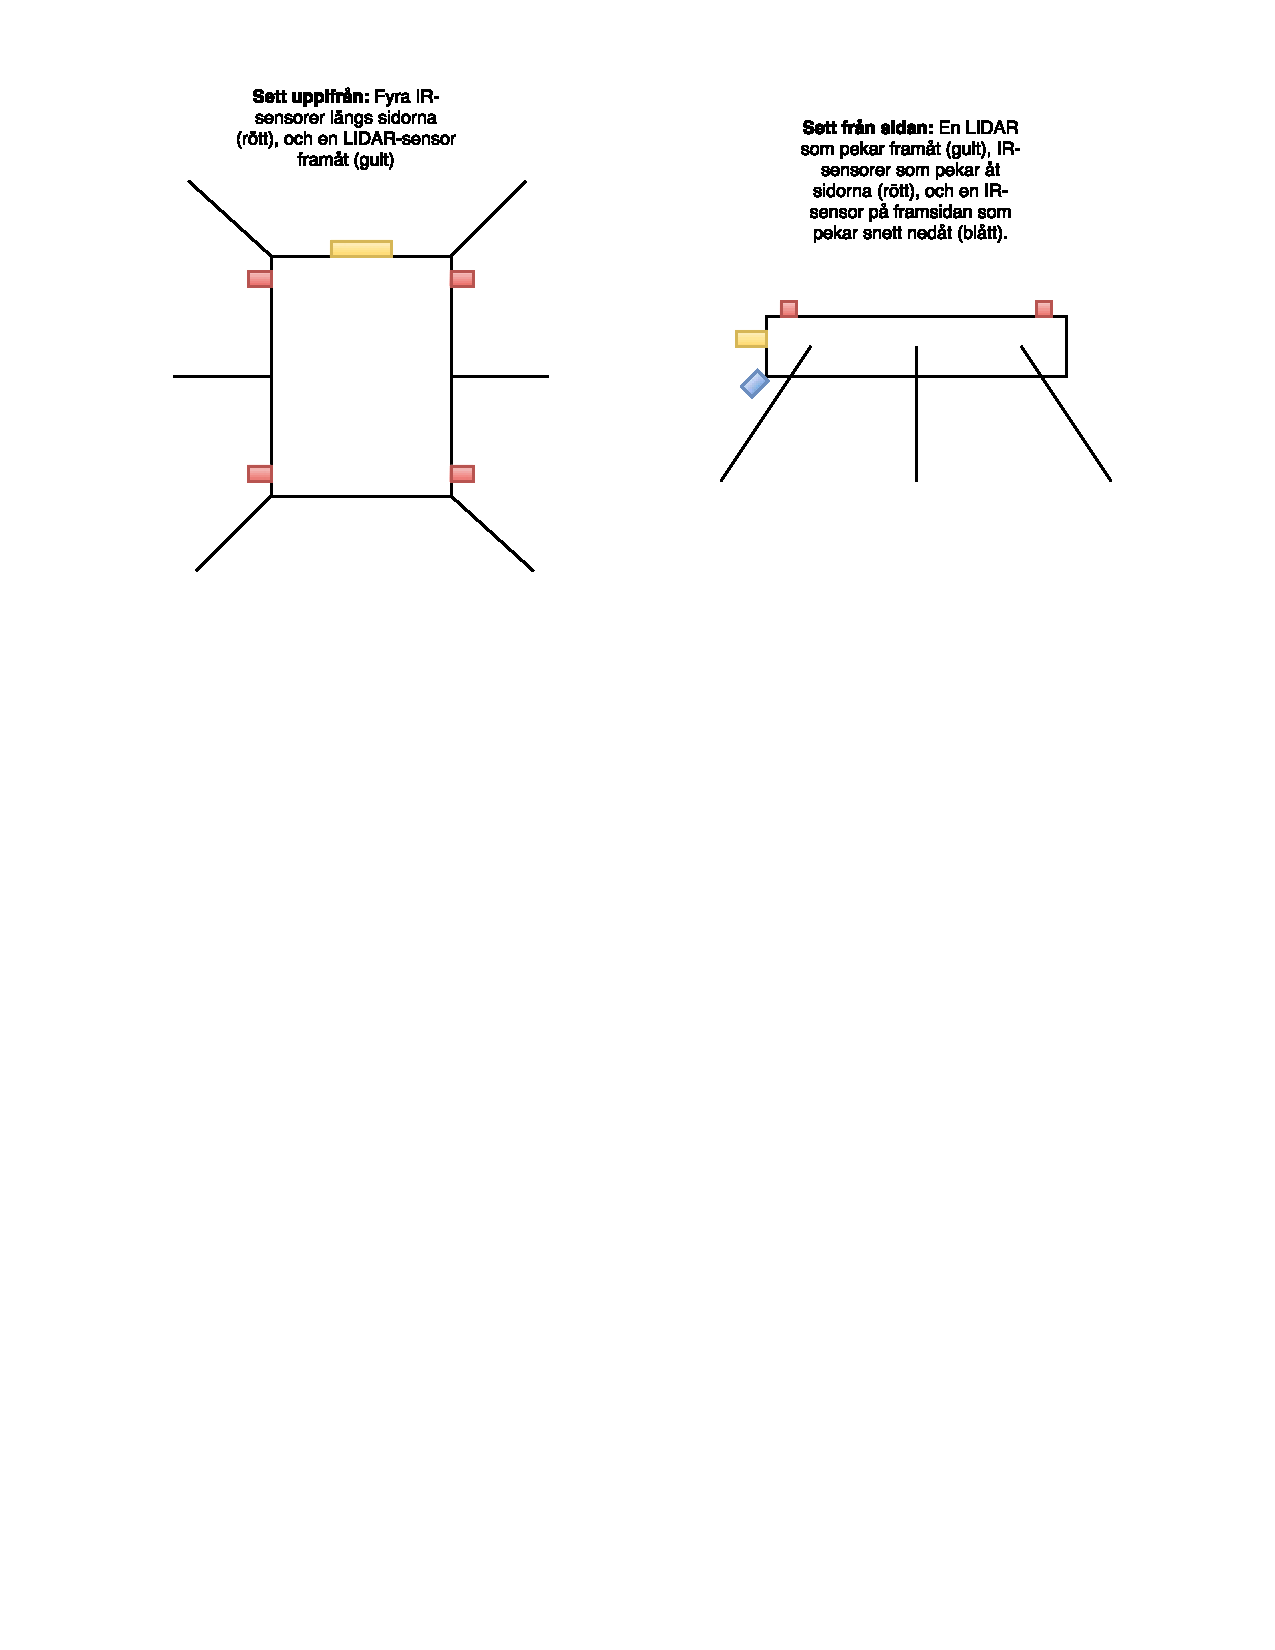
\includegraphics[width=17cm, trim=2cm 18cm 0cm 0cm]{images/sensor_mount.pdf}
        \caption{Montering av avståndssensorer\label{fig:sensor_mount}}
    \end{figure}

    \newpage
    \subsection{Krets}

    \begin{figure}[h]
        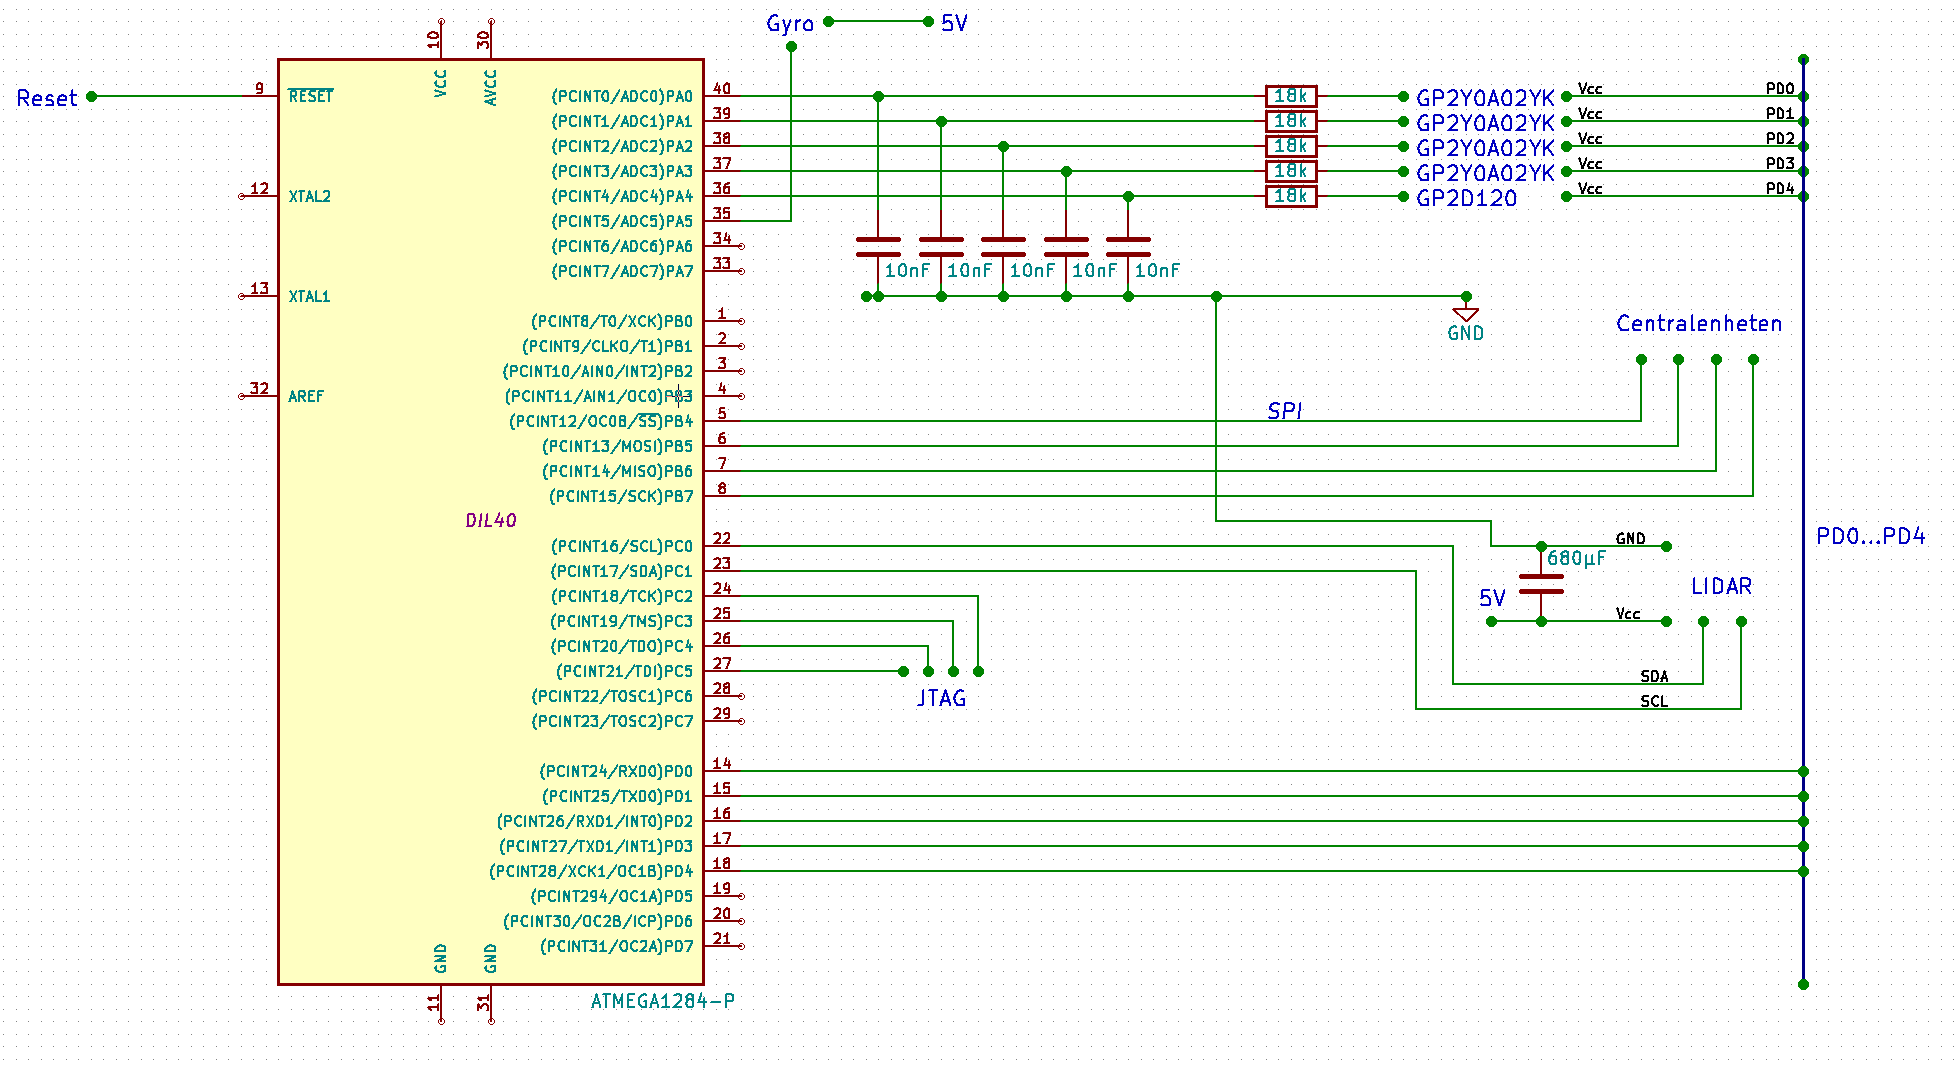
\includegraphics[width=15cm]{images/schematic_sensor.png}
        \caption{Kretschema över sensorenheten\label{fig:schem_sensor}}
    \end{figure}

    Ett antal lågpass-filter används för filtrering av brus från IR-sensorerna
    och utgörs av en kondenstator på 10nF och en 18kOhm-resistor för varje
    sensor. Filtret är kopplad mellan sensorerna och de analoga PA-ingångarna på
    processorn.

    LIDAR-sensorn är ansluten via PWM till PD5 på processorn.

    PC2 upp till PC5 används som anslutning till JTAG, för programmering av
    processorn, och PB4 upp till PB7 är anslutna via SPI till centralenheten.

    Figur \ref{fig:schem_sensor} visar ett kretschema över sensorenheten.

	
	%%%%%%%%%%%%%%%%%%%%%%%%%%%%%%%%%%%%%%%%%%%%%%%%%%%%%%%%%%%%%%%%%%%%%%%%%%%%%%%%%
	%						Grafiskt användargränssnitt
	%%%%%%%%%%%%%%%%%%%%%%%%%%%%%%%%%%%%%%%%%%%%%%%%%%%%%%%%%%%%%%%%%%%%%%%%%%%%%%%%%

    \newpage
	\section{Grafiskt användargränssnitt}
	På centralenheten körs en webbserver som tillhandahåller ett gränssnitt för
    användaren där man kan läsa sensordata eller kontrollera roboten i manuellt
    läge. Front-end-delen är skriven i Elm och back-end-delen i Elixir med hjälp
    av webbramverket Phoenix. På webbservern körs också RabbitMQ som används som
    en kommunikationsserver mellan centralenheten och webbservern/gui:t. Se
    \ref{gui:kommunikation} Kommunikation nedan.

	I det manuella läget styrs roboten med en joystick som är kopplad till
    användarens dator eller med knappar på gränssnittet. Figur
    \ref{fig:gui-overview} visar en illustration av det grafiska gränssnittet.
	
	\begin{figure}[h]
		\centering
		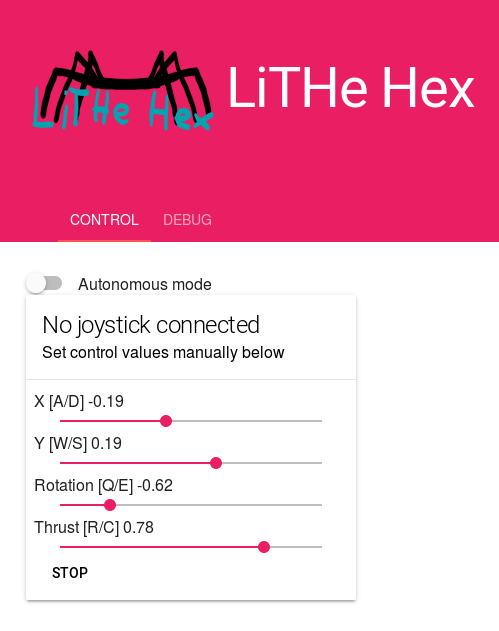
\includegraphics[width=0.5\linewidth]{images/gui-index.png}
		\caption{Det grafiska gränssnittet\label{fig:gui-overview}}
	\end{figure}

	\subsection{Webbserver}
	Webbservern är skriven i Elixir och använder webbramverket Phoenix.
    Kommunikationen mellan frontend och backend sker via en channel. En channel
    är en socket som tillåter kommunikation mellan en klient och en server. I
    channeln så skickas det från frontend till backend styrdata, d.v.s,
    joystickdata och om det autonoma läget ska köras eller inte. Från backend
    till frontend skickas debugdata som IR-sensorer, LIDAR samt vinklar.
	
	Backend skickar styrdata till RabbitMQ servern som centralenheten sedan
	läser av. Det skickas varje 0.5 sekund till RabbitMQ servern.

    \subsection{Styrning}
    Under styrning kan man välja om roboten ska köras autonomt eller i manuellt läge.
    För att ändra vilket läge roboten ska köras i finns en knapp som växlar dess läge.
    
    \subsubsection{Autonomt läge}
    Användaren klickar på en knapp som då sätter roboten i autonomt läge. Detta beskrivs i sektion \ref{sec:central-autonom}.
    
    \subsubsection{Manuell Styrning}
    Under styrning man man styra roboten med en joystick. Man kan även
    styra roboten med knappar/reglage på skärmen. Med de kan man styra
    roboten som då säger åt roboten att gå i en riktning,
    att vrida sig åt ett håll eller att stanna.

    \subsection{Debug}
	Under debug visas robotens olika inställningar samt sensordata vid
    tillfället. Sidan uppdateras 10 gånger per sekund och klienten får den
    uppdaterade data:n med hjälp av JSON. Det finns också flera grafer
    som beskriver några av de olika sensorernas data. Man kan också ändra
    styrparametrarna till regleralgoritmen.

	\label{gui:kommunikation}
    \subsection{Kommunikation}

	\begin{longtable}[c]{l l l }
        \textbf{Data} & \textbf{Nyckel} & \textbf{Typ} \\ \midrule
        IR-sensor ned & "ir\_down" & float \\
        IR-sensor fram vänster & "ir\_fl" & float \\
        IR-sensor fram höger & "ir\_fr" & float \\
        IR-sensor bak vänster & "ir\_bl" & float \\
        IR-sensor bak höger & "ir\_br" & float \\
        LIDAR & "lidar" & float \\
        Vinkel till vänster vägg & "angle\_l" & float \\
        Vinkel till höger vägg & "angle\_r" & float \\
        Genomsnittlig vinkel & "angle\_avg" & float \\
        Självgående läge & "auto" & bool \\
        Debugsträng & "debug" & string \\

		\caption{Format på JSON-strängen från
        centralenheten\label{table:guimessagesfromcentral}}
	\end{longtable}

	\begin{longtable}[c]{l l l }
        \textbf{Data} & \textbf{Nyckel} & \textbf{Typ} \\ \midrule
        X-hastighet & "x" & float \\
        Y-hastighet & "y" & float \\
        Rotation & "rotation" & float \\
        Thrust & "thrust" & float \\
        Självgående läge & "auto" & bool \\

		\caption{Format på JSON-strängen till
        centralenheten\label{table:guimessagestocentral}}
	\end{longtable}
    

	%%%%%%%%%%%%%%%%%%%%%%%%%%%%%%%%%%%%%%%%%%%%%%%%%%%%%%%%%%%%%%%%%%%%%%%%%%%%%%%%%
	%						Simuleringar
	%%%%%%%%%%%%%%%%%%%%%%%%%%%%%%%%%%%%%%%%%%%%%%%%%%%%%%%%%%%%%%%%%%%%%%%%%%%%%%%%%
    \newpage
	\section{Simuleringar}
	För att underlätta utvecklingen av vissa delar av projektet har vi att
    skrivit kod för att simulera dessa delar. Simuleringarna kör samma kod som
    ska köras på roboten men visualisera resultatet utan resten av roboten. De
    delar där simulering är mest aktuellt är inverterad kinematik,
    korridorföljning och gångstil.

	\subsection{Simulering för inverterad kinematik}
	Simuleringen går till genom att implementera algoritmen för 2D som beskrivs
    i avsnitt \ref{sub:inverterad-kinematik}. Simuleringen ritas sedan ut i
    webbläsaren för att visualisera den inverterade kinematiken. Den här
    simuleringen är skriven i Elm.
	
	\subsection{Simulering för korridorföljning}
	Simulering för korridorföljning kan testa olika regleralgoritmer utan att
    behöva testa dem på en gående robot. Simuleringen ritar ut en korridor och
    en robot som går framåt. Simulatorn skickar ut sensorvärden till en fil,
    regleralgoritmen läser in sensorvärden och tar sedan beslut. Roboten i
    simulatorn använder två IR-sensorer på varje sida som pekar rakt ut från
    roboten, det går att välja var på roboten som sensorerna ska sitta. Beslutet
    av regleralgoritmen skrivs till en fil som simulatorn läser in och styr
    roboten efter det. Det finns möjlighet att lägga till en störningsfunktion
    som till exempel kan vara att roboten alltid går med en liten rotation.
	
	\subsection{Simulering för gångstil}
	Simulatorn för gångstil fungerar på samma sätt som
    korridorföljningssimulatorn. Motorikenhetens kod skriver informationen som
    på roboten skulle skickas till servona till en fil som simulatorn läser.
    Simulatorn visualiserar resultatet av kommandona och skriver data som
    servona skulle svara med till en annan fil som motorikkoden kan läsa.

	\section{Slutsatser}
	Vilka förbättringar skulle kunna göras?

	\appendix
	\section{Kopplingsschema}
	HÄR VAR DET SCHEMAN
	
	\section{Programlistning}
	Här visas en lista på de olika program roboten
	använder sig av.
	
	\begin{longtable}[c]{l l l l}
		\textbf{Program} & \textbf{Programmerare} & \textbf{Datum}& \textbf{Version} \\ \midrule
		Inverterad Kinematik & Emil Segerbäck, Hannes Tuhkala & 2016-12-02 & 1.0 \\
		Gångstil & Olav Övrebö & 2016-12-13 & 1.0 \\ 
		Kommunikation med SPI & Malcolm Vigren, Noak Ringman & 2016-12-13 & 1.0 \\ 
		Webbserver/GUI & Emil Segerbäck, Hannes Tuhkala & 2016-12-13 & 1.0 \\ 
		Beslutsfattning & Robin Sliwa, Noak Ringman & 2016-12-13 & 1.0 \\ 
		PID-reglering & Robin Sliwa, Olav Övrebö & 2016-12-13 & 1.0 \\ 
		Motorik & Olav Övrebö, Frans Skarman & 2016-12-13 & 1.0 \\ 
		Servokontroll & Frans Skarman & 2016-12-13 & 1.0 \\ 
		Sensorenheten & Malcolm Vigren, Noak Ringman & 2016-12-01 & 1.0 \\
		
		\caption{Lista över program \label{table:programlisting}}
	\end{longtable}
	
	\section{Övrigt}
	HÄR VAR DET ÖVRIGT
	
	\addtocontents{toc}
	
\end{document}
